% !TeX program = pdflatex
% Rapport de projet professionnel — Tradivia System
% Compiler deux fois : pdflatex rapport_tradivia.tex
% Personnaliser les commandes ci-dessous avant le dépôt.
\documentclass[12pt,a4paper,oneside]{report}

% ---------- Encodage, langue et typographie ----------

\usepackage[utf8]{inputenc}
\usepackage[T1]{fontenc}
\usepackage[english,main=french,provide=*]{babel}
\usepackage{lmodern}
\usepackage{microtype}
\usepackage{setspace}
\onehalfspacing



% ---------- Mise en page ----------
\usepackage[a4paper,top=2.4cm,bottom=2.4cm,left=2.8cm,right=2.4cm]{geometry}
\usepackage{fancyhdr}
\usepackage{titlesec}
\usepackage{xcolor}
\usepackage{enumitem}
\usepackage{emptypage}
\usepackage{lastpage}



% ---------- Tableaux, figures et code ----------
\usepackage{graphicx}
\usepackage{float}
\usepackage{booktabs}
\usepackage{tabularx}
\usepackage{longtable}
\usepackage{array}
\usepackage{multirow}
\usepackage{caption}
\usepackage{subcaption}
\usepackage{listings}
\usepackage{tikz}
\usetikzlibrary{arrows.meta,positioning,shapes.geometric,fit,calc}
\usepackage{pgfgantt}

% ---------- Mathématiques, liens et glossaire ----------
\usepackage{amsmath,amssymb}
\usepackage{url}
\usepackage{hyperref}
\usepackage{bookmark}

% ---------- Informations à personnaliser ----------
\newcommand{\Etablissement}{Nom de l'établissement}
\newcommand{\Departement}{Département Informatique}
\newcommand{\Filiere}{Filière Génie Logiciel et Systèmes d'Information}
\newcommand{\Auteur}{Nom et prénom de l'étudiant(e)}
\newcommand{\Encadrant}{Nom de l'encadrant(e)}
\newcommand{\AnneeUniversitaire}{2025--2026}
\newcommand{\TitreProjet}{Conception et réalisation d'un système de gestion commerciale pour TRADIVIA}

% ---------- Couleurs et styles ----------
\definecolor{tradiviablue}{HTML}{123B5D}
\definecolor{tradiviagold}{HTML}{D79A2B}
\definecolor{lightblue}{HTML}{EAF2F8}
\definecolor{codegray}{HTML}{F5F5F5}
\hypersetup{colorlinks=true,linkcolor=tradiviablue,urlcolor=tradiviablue,citecolor=tradiviablue,pdftitle={Rapport Tradivia System},pdfauthor={\Auteur}}
\setlist[itemize]{label=\textcolor{tradiviagold}{\textbullet},leftmargin=1.2cm}
% Page d'ouverture réservée à chaque chapitre numéroté.
\titleformat{\chapter}[display]
  {\thispagestyle{empty}\normalfont\bfseries\centering\color{tradiviablue}}
  {\Large Chapitre \thechapter}
  {1.5ex}
  {\titlerule\vspace{1.4cm}\Huge}
  [\vspace{1.4cm}\textcolor{tradiviagold}{\rule{0.34\textwidth}{2pt}}\thispagestyle{empty}\clearpage]
\titlespacing*{\chapter}{0pt}{0.28\textheight}{0pt}
% Les chapitres non numérotés gardent une présentation compacte.
\titleformat{name=\chapter,numberless}[display]
  {\normalfont\bfseries\color{tradiviablue}}
  {}
  {0pt}
  {\Huge}
\titlespacing*{name=\chapter,numberless}{0pt}{0pt}{1.5cm}
\titleformat{\section}{\Large\bfseries\color{tradiviablue}}{\thesection}{0.8em}{}
\titleformat{\subsection}{\large\bfseries\color{tradiviablue}}{\thesubsection}{0.8em}{}
\pagestyle{fancy}
\setlength{\headheight}{25pt}
\fancyhf{}

% Afficher uniquement le numéro et le nom du chapitre.
\renewcommand{\chaptermark}[1]{%
  \markboth{Chapitre \thechapter.\ #1}{}%
}

\fancyhead[C]{%
  \small\textcolor{tradiviablue}{\nouppercase{\leftmark}}%
}

\fancyfoot[C]{\small Page \thepage\ sur \pageref{LastPage}}

\renewcommand{\headrulewidth}{0.5pt}
\renewcommand{\headrule}{%
  \hbox to\headwidth{%
    \color{tradiviagold}%
    \leaders\hrule height \headrulewidth\hfill
  }%
}

% ---------- Code, tableaux et illustrations ----------
\lstset{
  backgroundcolor=\color{codegray},
  basicstyle=\ttfamily\small,
  breaklines=true,
  frame=single,
  rulecolor=\color{tradiviablue},
  numbers=left,
  numberstyle=\tiny\color{gray},
  showstringspaces=false,
  tabsize=2,
  captionpos=b
}
\newcolumntype{Y}{>{\raggedright\arraybackslash}X}
\newcommand{\code}[1]{\texttt{#1}}
\graphicspath{{figures/}}

% Par défaut, une illustration absente est seulement signalée dans le journal.
% Dans le chapitre 5, \showmissingfigurestrue affiche à la place un cadre.
\newif\ifshowmissingfigures
\showmissingfiguresfalse
\newcommand{\projectfigure}[3][6.2cm]{%
  \IfFileExists{figures/#2}{%
    \begin{figure}[H]
      \centering
      \includegraphics[width=0.92\textwidth,height=#1,keepaspectratio]{#2}%
      \caption{#3}
    \end{figure}%
  }{%
    \ifshowmissingfigures
      \begin{figure}[H]
        \centering
        \fbox{%
          \begin{minipage}[c][#1][c]{0.88\textwidth}
            \centering
            \textcolor{tradiviablue}{\Large\bfseries Capture d'écran à insérer}\par
            \vspace{0.45cm}
            \small Fichier attendu : \texttt{figures/#2}
          \end{minipage}%
        }
        \caption{#3}
      \end{figure}%
    \else
      \PackageWarning{tradivia}{Illustration `figures/#2' introuvable}%
    \fi
  }%
}
\begin{document}

% =====================================================
% PAGE DE GARDE
% =====================================================
\begin{titlepage}
\begin{center}
{\large Royaume du Maroc}\par
\vspace{0.3cm}
{\Large\bfseries \Etablissement}\par
{\large \Departement}\par
{\large \Filiere}\par
\vspace{1.2cm}
\textcolor{tradiviablue}{\rule{\textwidth}{1.2pt}}\par
\vspace{0.6cm}
{\LARGE\bfseries Rapport de projet professionnel}\par
\vspace{0.7cm}
{\Huge\bfseries\color{tradiviablue}\TitreProjet}\par
\vspace{0.5cm}
\textcolor{tradiviagold}{\rule{0.75\textwidth}{2pt}}\par
\vfill
\begin{tabularx}{0.9\textwidth}{Y Y}
\textbf{Réalisé par :} & \textbf{Encadré par :}\\[0.3cm]
\Auteur & \Encadrant\\
\end{tabularx}
\vfill
{\large Année universitaire : \AnneeUniversitaire}
\end{center}
\end{titlepage}

\pagenumbering{roman}
\setcounter{page}{2}

\chapter*{Remerciements}
\addcontentsline{toc}{chapter}{Remerciements}
Je tiens à exprimer ma profonde gratitude à toutes les personnes qui ont contribué à la réalisation de ce projet. Je remercie également l'équipe de TRADIVIA pour la confiance accordée, la présentation de ses procédures commerciales et comptables, ainsi que la disponibilité dont elle a fait preuve lors de l'identification et de la validation des besoins. Cette collaboration a permis de construire une solution cohérente avec les activités réelles de l'entreprise.

J'adresse enfin mes sincères remerciements aux enseignants, aux membres du jury, à mes collègues, à mes amis et à ma famille pour leur soutien, leur patience et leurs encouragements.

\chapter*{Résumé}
\addcontentsline{toc}{chapter}{Résumé}
La gestion quotidienne d'une entreprise commerciale exige la centralisation d'informations hétérogènes : clients, factures, règlements, expéditions, dépenses, déclarations de taxe sur la valeur ajoutée et documents administratifs. Lorsque ces données sont réparties entre fichiers, documents papier et outils non intégrés, le risque d'erreur augmente et le suivi de l'activité devient difficile.

Ce projet présente la conception et la réalisation de \textbf{Tradivia System}, une application web locale destinée à numériser et unifier les principales opérations de TRADIVIA. La solution permet de gérer les clients, les factures et leurs paiements, les conteneurs et leurs pièces jointes, les charges, les ordres de virement, ainsi que des indicateurs comptables et fiscaux. Elle automatise également la génération de documents Word et PDF à partir de modèles métier.

L'application repose sur un frontend développé avec React et Vite, une API REST Express, une base SQLite et des scripts Python utilisant \code{python-docx} et l'automatisation Microsoft Word. L'accès est protégé par des jetons JWT et les mots de passe sont hachés avec bcrypt. Le résultat est un outil centralisé, simple à déployer sur Windows et adapté aux besoins d'une petite structure commerciale.

\textbf{Mots-clés :} gestion commerciale, React, Express, SQLite, JWT, facturation, comptabilité, génération documentaire.

\begin{otherlanguage}{english}
\chapter*{Abstract}
\addcontentsline{toc}{chapter}{Abstract}
The daily management of a trading company requires the centralization of heterogeneous information such as customers, invoices, payments, shipments, expenses, value-added tax declarations and administrative documents. When these data are scattered across files, paper documents and unrelated tools, errors become more likely and business monitoring becomes difficult.

This report presents the design and implementation of \textbf{Tradivia System}, a local web application that digitizes and unifies TRADIVIA's main operations. The solution manages customers, invoices and payments, containers and attached files, expenses, VAT transfer orders, as well as accounting and tax indicators. It also automates Word and PDF document generation from business templates.

The system uses React and Vite for the frontend, an Express REST API, a SQLite database, and Python scripts based on \code{python-docx} and Microsoft Word automation. Access is protected through JWT tokens and passwords are hashed with bcrypt. The resulting solution is centralized, easy to deploy on Windows and appropriate for a small trading organization.

\textbf{Keywords:} business management, React, Express, SQLite, JWT, invoicing, accounting, document generation.
\end{otherlanguage}

\chapter*{Introduction générale}
\addcontentsline{toc}{chapter}{Introduction générale}
La transformation numérique ne concerne plus uniquement les grandes organisations. Une petite ou moyenne entreprise doit elle aussi disposer d'informations fiables, rapidement accessibles et cohérentes pour suivre ses ventes, ses dépenses et ses engagements. Dans une activité commerciale intégrant des opérations d'importation, le volume documentaire et la diversité des traitements rendent cette exigence encore plus importante.

Avant la mise en place de Tradivia System, les informations nécessaires au pilotage pouvaient être réparties entre plusieurs supports. Une facture devait être créée, classée, suivie jusqu'au règlement puis prise en compte dans les calculs comptables. De même, chaque conteneur devait être associé à ses dates, références et documents. Cette dispersion ralentit le travail, complique les recherches et favorise les doubles saisies.

Le projet a donc pour finalité de concevoir une application locale qui centralise le cycle commercial et administratif de TRADIVIA. La solution doit rester simple d'utilisation, fonctionner sur un ordinateur Windows et générer les documents déjà utilisés par l'entreprise. Elle doit aussi fournir une vision synthétique du chiffre d'affaires, des charges, de la TVA et des estimations fiscales.

Le présent rapport expose successivement la spécification des besoins, l'organisation du projet, la modélisation du système, les choix d'implémentation et les principales interfaces réalisées. Il se termine par un bilan, les limites observées et les perspectives d'évolution.

\chapter*{Liste des abréviations}
\addcontentsline{toc}{chapter}{Liste des abréviations}
\begin{longtable}{p{3cm}p{11cm}}
\textbf{API} & Application Programming Interface\\
\textbf{CRUD} & Create, Read, Update, Delete\\
\textbf{CORS} & Cross-Origin Resource Sharing\\
\textbf{CSS} & Contribution sociale de solidarité ; selon le contexte web, Cascading Style Sheets\\
\textbf{DOCX} & Format de document Microsoft Word Open XML\\
\textbf{HTTP} & HyperText Transfer Protocol\\
\textbf{HT} & Hors taxes\\
\textbf{IS} & Impôt sur les sociétés\\
\textbf{JWT} & JSON Web Token\\
\textbf{MCD} & Modèle conceptuel de données\\
\textbf{MLD} & Modèle logique de données\\
\textbf{PDF} & Portable Document Format\\
\textbf{REST} & Representational State Transfer\\
\textbf{SGBD} & Système de gestion de base de données\\
\textbf{SPA} & Single Page Application\\
\textbf{SQL} & Structured Query Language\\
\textbf{TTC} & Toutes taxes comprises\\
\textbf{TVA} & Taxe sur la valeur ajoutée\\
\textbf{UI/UX} & User Interface / User Experience\\
\textbf{UML} & Unified Modeling Language\\
\end{longtable}

\tableofcontents
\listoffigures
\listoftables
\clearpage
\pagenumbering{arabic}

% =====================================================
\chapter{Spécification des besoins}
% =====================================================
\section*{Introduction}
\addcontentsline{toc}{section}{Introduction}
Ce chapitre définit le contexte, la problématique, les objectifs et le cahier des charges de Tradivia System. Il distingue les besoins fonctionnels des exigences de qualité et délimite le périmètre retenu.

\section{Contexte du projet}
TRADIVIA exerce une activité commerciale nécessitant le suivi simultané des ventes, des clients, des marchandises transportées par conteneurs, des charges et des obligations comptables. Une opération ne produit pas seulement une ligne de données : elle entraîne des justificatifs, des références, des échéances et parfois un document officiel à générer.

L'entreprise a besoin d'une solution utilisable localement, sans infrastructure complexe, capable de conserver l'historique des opérations et de produire rapidement des documents homogènes. Le système doit également réduire la dépendance aux calculs manuels et donner une lecture consolidée des résultats annuels.

\subsection{Étude de l'existant}
Avant le développement d'un système unifié, une petite structure commerciale s'appuie généralement sur une combinaison de feuilles de calcul, documents Word, dossiers de fichiers et échanges informels. Cette organisation peut répondre à un faible volume, mais elle atteint rapidement ses limites : une modification doit être reportée dans plusieurs supports, les versions de documents se multiplient et la recherche d'une pièce dépend de la personne qui l'a classée.

Dans le contexte de TRADIVIA, les informations commerciales et logistiques sont étroitement liées. Le règlement d'une facture influence les créances ; une charge influence la TVA déductible et le résultat ; un conteneur regroupe plusieurs documents de transport. L'absence de référentiel commun rend donc les contrôles transversaux difficiles.

\begin{table}[H]\centering
\caption{Analyse synthétique de l'existant}
\begin{tabularx}{\textwidth}{Y Y Y}
\toprule \textbf{Pratique} & \textbf{Avantage initial} & \textbf{Limite observée}\\ \midrule
Fichiers bureautiques séparés & Mise en œuvre immédiate & Doublons, versions concurrentes et consolidation manuelle\\
Classement par dossiers & Organisation familière & Recherche lente et absence de lien direct avec l'opération\\
Calculs manuels & Flexibilité ponctuelle & Risque d'erreur et difficulté de reproduction\\
Suivi informel des règlements & Peu de saisie & Vision imprécise des créances\\
Documents rédigés un par un & Liberté de mise en forme & Temps de préparation et incohérences typographiques\\
\bottomrule
\end{tabularx}
\end{table}

\subsection{Justification de React et Vite}
React permet de composer l'interface à partir d'états et de composants réutilisables. Cette approche convient aux listes interactives, formulaires modaux, filtres et indicateurs qui doivent se mettre à jour sans recharger toute la page. Vite apporte un démarrage rapide en développement, le remplacement à chaud et une compilation de production simple.

Le projet actuel rassemble encore une grande partie de l'interface dans \code{App.jsx}. Ce choix a accéléré le prototype, mais ne remet pas en cause la pertinence de React. Une évolution naturelle consistera à extraire les composants par domaine et à introduire un routeur.

\subsection{Justification d'Express}
Express offre un modèle minimal pour déclarer les routes et les middlewares. Il s'intègre directement aux bibliothèques nécessaires au projet : JWT, bcrypt, Multer et better-sqlite3. Utiliser JavaScript sur le frontend et le backend réduit également le nombre de langages nécessaires pour les traitements web courants.

\subsection{Justification de SQLite}
SQLite stocke l'ensemble de la base dans un fichier, ne nécessite aucun service et fournit les transactions, contraintes d'unicité et clés étrangères attendues. Pour une application locale utilisée par une petite équipe, ce compromis réduit considérablement l'administration. Une base serveur deviendrait préférable en cas d'accès simultanés nombreux, de réplication ou de disponibilité distante.

\subsection{Comparaison des solutions envisagées}
\begin{table}[H]\centering
\caption{Comparaison de quelques choix technologiques}
\begin{tabularx}{\textwidth}{p{3cm}Y Y Y}
\toprule \textbf{Critère} & \textbf{Choix retenu} & \textbf{Alternative} & \textbf{Décision}\\ \midrule
Interface & React & Application de bureau & Interface web plus facile à faire évoluer\\
API & REST/Express & GraphQL & Ressources CRUD simples, REST suffisant\\
Base locale & SQLite & PostgreSQL & Administration minimale pour le volume actuel\\
Documents & Python/Word & Génération PDF native & Fidélité aux modèles Word existants\\
Authentification & JWT & Session serveur & API stateless simple pour le poste local\\
\bottomrule
\end{tabularx}
\end{table}

\subsection{Solution proposée}
La solution proposée est une application web locale accessible depuis un navigateur. Toutes les opérations sont enregistrées dans une base SQLite unique. L'interface présente les fonctions par domaine, tandis que l'API applique les règles de calcul et assure la persistance. Les documents de conteneurs sont conservés sur disque avec leurs métadonnées en base, et les documents officiels sont générés à partir de modèles Word contrôlés.

Ce choix conserve la simplicité d'un logiciel installé sur un poste Windows tout en bénéficiant de l'ergonomie d'une interface web. Il permet aussi une évolution progressive : la base locale pourrait ultérieurement être remplacée par un serveur de données sans remettre en cause l'ensemble de l'expérience utilisateur.

\section{Problématique}
La question directrice du projet est la suivante :

\begin{quote}
\textit{Comment concevoir une application locale, sécurisée et ergonomique qui centralise la gestion commerciale, logistique, documentaire et comptable de TRADIVIA tout en automatisant la production de ses documents Word et PDF ?}
\end{quote}

Cette problématique recouvre plusieurs difficultés : dispersion des informations, incohérences entre documents et données, suivi manuel des paiements, classement des pièces de conteneurs, répétition des calculs de TVA et absence d'une vision synthétique de l'activité.

\section{Objectifs du projet}
\subsection{Objectif général}
L'objectif général est de mettre à disposition de TRADIVIA un système d'information intégré pour enregistrer, consulter et exploiter ses données commerciales depuis une interface web unique.

\subsection{Objectifs spécifiques}
\begin{itemize}
  \item sécuriser l'accès par authentification et gestion de rôles ;
  \item centraliser les fiches clients et éviter les ressaisies ;
  \item automatiser le calcul, l'enregistrement et l'export des factures ;
  \item suivre l'état payé ou impayé des factures ;
  \item suivre les conteneurs, leurs itinéraires et leurs documents ;
  \item enregistrer et analyser les charges par catégorie et période ;
  \item gérer les ordres de virement TVA et ZIZI ;
  \item produire des tableaux de bord comptables et des estimations fiscales ;
  \item clôturer et historiser les exercices comptables ;
  \item générer des documents DOCX et PDF conformes aux modèles de l'entreprise.
\end{itemize}

\subsection{Critères de réussite}
Le projet est considéré comme réussi si un utilisateur authentifié peut effectuer les opérations quotidiennes sans recourir à un second outil pour les calculs principaux. Les critères de validation sont notamment la création d'une facture correcte, son export fidèle, le suivi de son paiement, l'association de fichiers à un conteneur, l'enregistrement d'une charge et l'obtention d'une synthèse comptable annuelle.

La réussite suppose également que les données persistent après le redémarrage, que les erreurs usuelles soient signalées clairement et qu'une procédure de sauvegarde permette de restaurer la base et les pièces jointes.

\section{Étude de faisabilité}
\subsection{Faisabilité technique}
Les technologies retenues sont compatibles avec Windows et disponibles librement, à l'exception de Microsoft Word déjà requis pour une conversion PDF fidèle aux modèles existants. React, Express et SQLite disposent d'écosystèmes matures. Python fournit une bibliothèque adaptée à la manipulation du format DOCX, et l'automatisation COM permet d'utiliser le moteur de rendu de Word.

\subsection{Faisabilité opérationnelle}
L'application s'exécute dans un navigateur et reprend le vocabulaire métier de l'entreprise : facture, client, conteneur, charge, TVA et exercice. Le coût d'apprentissage est ainsi limité. Les données restent sur le poste local, ce qui facilite l'adoption dans une organisation ne disposant pas d'une infrastructure serveur permanente.

\subsection{Faisabilité économique}
Le socle logiciel est principalement open source et ne nécessite pas d'abonnement applicatif. Les coûts concernent surtout le temps de développement, le poste Windows, Microsoft Word et la mise en place d'une politique de sauvegarde. Pour le volume visé, SQLite évite l'administration d'un serveur de base de données.

\section{Acteurs du système}
\begin{table}[H]\centering
\caption{Acteurs et responsabilités}
\begin{tabularx}{\textwidth}{p{3cm}Y}
\toprule
\textbf{Acteur} & \textbf{Responsabilités}\\
\midrule
Administrateur & Authentification, gestion des utilisateurs, accès à toutes les fonctions métier, création et désactivation de comptes.\\
Utilisateur & Gestion des clients, factures, conteneurs, charges, virements, exports et consultation de la comptabilité.\\
Microsoft Word & Conversion automatisée des documents DOCX vers PDF sous Windows.\\
Système de fichiers & Conservation des pièces jointes des conteneurs et des modèles Word.\\
\bottomrule
\end{tabularx}
\end{table}

\section{Cahier des charges}
\subsection{Besoins fonctionnels}
\begin{longtable}{p{2cm}p{4cm}p{8cm}}
\caption{Besoins fonctionnels principaux}\label{tab:bf}\\
\toprule \textbf{ID} & \textbf{Module} & \textbf{Besoin}\\ \midrule
\endfirsthead
\toprule \textbf{ID} & \textbf{Module} & \textbf{Besoin}\\ \midrule
\endhead
BF01 & Authentification & Se connecter, valider la session et changer son mot de passe.\\
BF02 & Utilisateurs & Créer, lister et désactiver des utilisateurs en tant qu'administrateur.\\
BF03 & Clients & Ajouter, modifier, rechercher et supprimer une fiche client.\\
BF04 & Factures & Créer, calculer, modifier, filtrer et supprimer une facture.\\
BF05 & Paiements & Marquer une facture comme payée ou impayée.\\
BF06 & Exports & Exporter une ou plusieurs factures en DOCX ou PDF.\\
BF07 & Conteneurs & Gérer les références, ports, dates, poids, sacs et statuts.\\
BF08 & Documents & Téléverser, afficher, télécharger et supprimer les pièces d'un conteneur.\\
BF09 & Charges & Enregistrer et analyser les dépenses par année, catégorie et fournisseur.\\
BF10 & Virements & Gérer et exporter les ordres TVA et ZIZI.\\
BF11 & Comptabilité & Afficher revenus, charges, marges, TVA, créances et tendances.\\
BF12 & Fiscalité & Estimer IS, cotisation minimale, CSS et patente.\\
BF13 & Exercices & Clôturer un exercice et conserver ses agrégats.\\
\bottomrule
\end{longtable}

\subsection{Besoins non fonctionnels}
\begin{itemize}
  \item \textbf{Ergonomie :} navigation homogène, formulaires explicites et filtres rapides.
  \item \textbf{Sécurité :} mots de passe hachés, session JWT de durée limitée, contrôle du rôle administrateur.
  \item \textbf{Fiabilité :} contraintes d'unicité, clés étrangères SQLite et validation des données sensibles.
  \item \textbf{Performance :} temps de réponse compatible avec une utilisation locale et un volume PME.
  \item \textbf{Maintenabilité :} code versionné, documentation technique et séparation frontend/API/scripts.
  \item \textbf{Portabilité :} fonctionnement sur Windows avec Node.js 20+, Python 3 et un navigateur récent.
  \item \textbf{Sauvegarde :} conservation conjointe de la base SQLite, des téléversements et des modèles.
\end{itemize}

\subsection{Scénarios fonctionnels prioritaires}
\paragraph{Créer et exporter une facture.}
L'utilisateur sélectionne un client existant ou choisit un client particulier, renseigne la date, la désignation, le prix et le mode de calcul. Le système détermine les montants, contrôle l'unicité du numéro, enregistre la facture et permet ensuite son export en DOCX ou PDF.

\paragraph{Suivre un conteneur.}
L'utilisateur crée la fiche logistique, complète les ports et dates, choisit un statut puis ajoute les justificatifs. Il peut filtrer la liste, ouvrir un document et mettre à jour l'état jusqu'à la livraison.

\paragraph{Analyser un exercice.}
L'utilisateur sélectionne l'année. Le système agrège ventes et charges, calcule la marge et la TVA, présente les tendances et propose des estimations fiscales. Au terme de l'exercice, une clôture conserve les valeurs calculées.

\subsection{Matrice de traçabilité}
\begin{table}[H]\centering
\caption{Correspondance entre objectifs, fonctions et validation}
\begin{tabularx}{\textwidth}{p{3.3cm}Y Y}
\toprule \textbf{Objectif} & \textbf{Fonction réalisée} & \textbf{Preuve attendue}\\ \midrule
Centraliser les ventes & Clients et factures & Facture enregistrée et retrouvée par filtre\\
Réduire les calculs manuels & Deux modes de calcul & Montants HT, TVA et TTC cohérents\\
Tracer la logistique & Conteneurs et documents & Fiche complète avec pièces consultables\\
Piloter les dépenses & Charges et statistiques & Totaux par catégorie et mois\\
Produire des documents & Scripts et modèles & Téléchargement DOCX/PDF\\
Suivre la situation & Module comptable & Indicateurs annuels et trimestriels\\
Sécuriser l'accès & JWT et rôles & Refus des requêtes sans jeton valide\\
\bottomrule
\end{tabularx}
\end{table}

\subsection{Contraintes techniques}
La solution doit fonctionner localement sur Windows. L'interface écoute sur le port 5173 et l'API sur le port 3001. La conversion PDF dépend de Microsoft Word et de \code{pywin32}. SQLite convient au contexte mono-poste ou petite équipe, mais ne vise pas une charge publique fortement concurrente.

\subsection{Livrables}
Les livrables sont le code source, la base de données initialisée, les modèles documentaires, les scripts de génération, les tests API, la documentation d'installation et le présent rapport.

\section*{Conclusion}
\addcontentsline{toc}{section}{Conclusion}
La spécification confirme qu'il ne s'agit pas d'un simple outil de facturation, mais d'un système transversal reliant commerce, logistique, documentation et comptabilité. Ces besoins structurent la planification et les modèles présentés dans les chapitres suivants.

% =====================================================
\chapter{Gestion du projet}
% =====================================================
\section*{Introduction}
\addcontentsline{toc}{section}{Introduction}
Une démarche incrémentale a été retenue afin de livrer en priorité les fonctions indispensables, puis d'ajouter les modules logistiques, comptables et documentaires.

\section{Cycle de vie}
Le projet suit une adaptation de la méthode Agile : recueil des besoins, constitution d'un backlog, conception, développement par incréments, validation et amélioration. Chaque incrément produit une fonction testable et réduit le risque de découvrir tardivement une erreur métier.

\begin{figure}[H]\centering
\begin{tikzpicture}[node distance=1.1cm and 0.8cm,box/.style={draw=tradiviablue,rounded corners,fill=lightblue,minimum width=2.5cm,minimum height=1cm,align=center},arr/.style={-Latex,thick,tradiviagold}]
\node[box] (b) {Besoins};
\node[box,right=of b] (c) {Conception};
\node[box,right=of c] (d) {Développement};
\node[box,below=of d] (t) {Tests};
\node[box,left=of t] (v) {Validation};
\node[box,left=of v] (a) {Amélioration};
\draw[arr] (b)--(c); \draw[arr] (c)--(d); \draw[arr] (d)--(t);
\draw[arr] (t)--(v); \draw[arr] (v)--(a); \draw[arr] (a)--(b);
\end{tikzpicture}
\caption{Cycle de développement incrémental}
\end{figure}

\section{Découpage des tâches}
\begin{table}[H]\centering
\caption{Découpage prévisionnel du projet}
\begin{tabularx}{\textwidth}{p{1.2cm}Y p{2cm}}
\toprule \textbf{Lot} & \textbf{Travaux} & \textbf{Durée}\\ \midrule
L1 & Analyse, inventaire des documents et cahier des charges & 1 semaine\\
L2 & Conception des données, architecture et maquettes & 2 semaines\\
L3 & Authentification, clients et factures & 3 semaines\\
L4 & Conteneurs, téléversements et charges & 3 semaines\\
L5 & Virements, génération Word/PDF et exports groupés & 2 semaines\\
L6 & Comptabilité, fiscalité et clôture & 2 semaines\\
L7 & Tests, corrections, documentation et livraison & 2 semaines\\
\bottomrule
\end{tabularx}
\end{table}

\section{Diagramme de Gantt}
\begin{figure}[H]\centering
\resizebox{\textwidth}{!}{%
\begin{ganttchart}[hgrid,vgrid,title/.style={fill=tradiviablue,draw=white},title label font=\color{white}\bfseries,bar/.style={fill=tradiviagold},bar label font=\small]{1}{15}
\gantttitle{Semaines}{15}\\
\gantttitlelist{1,...,15}{1}\\
\ganttbar{Analyse}{1}{1}\\
\ganttbar{Conception}{2}{3}\\
\ganttbar{Clients et factures}{4}{6}\\
\ganttbar{Conteneurs et charges}{7}{9}\\
\ganttbar{Documents et virements}{10}{11}\\
\ganttbar{Comptabilité}{12}{13}\\
\ganttbar{Tests et documentation}{14}{15}
\end{ganttchart}}
\caption{Planning indicatif de réalisation}
\end{figure}

\section{Ordonnancement PERT}
Le réseau PERT met en évidence les dépendances entre les lots. L'analyse des besoins précède nécessairement la conception des données. Le développement du socle doit être achevé avant les modules métier, alors que la documentation peut évoluer parallèlement aux tests. Le chemin critique passe par l'analyse, la conception, le socle, la facturation, la comptabilité et la recette finale.

\begin{figure}[H]\centering
\begin{tikzpicture}[node distance=1.4cm and 1.2cm,event/.style={draw=tradiviablue,circle,fill=lightblue,minimum size=1.05cm,font=\bfseries},task/.style={-Latex,thick,tradiviagold}]
\node[event] (d) {D};
\node[event,right=of d] (a) {A};
\node[event,right=of a] (c) {C};
\node[event,right=of c] (s) {S};
\node[event,above right=of s] (f) {F};
\node[event,below right=of s] (l) {L};
\node[event,right=3.1cm of s] (k) {K};
\node[event,right=of k] (t) {T};
\draw[task] (d)--node[above]{Besoins}(a);
\draw[task] (a)--node[above]{Conception}(c);
\draw[task] (c)--node[above]{Socle}(s);
\draw[task] (s)--node[above left]{Factures}(f);
\draw[task] (s)--node[below left]{Logistique}(l);
\draw[task] (f)--node[above right]{Comptabilité}(k);
\draw[task] (l)--node[below right]{Documents}(k);
\draw[task] (k)--node[above]{Tests}(t);
\end{tikzpicture}
\caption{Réseau PERT simplifié du projet}
\end{figure}

\section{Matrice RACI}
La matrice RACI clarifie qui réalise une tâche (R), qui en porte la responsabilité finale (A), qui est consulté (C) et qui doit être informé (I). Dans un projet individuel, l'étudiant cumule naturellement plusieurs responsabilités, mais l'encadrant et le représentant métier conservent des rôles de validation distincts.

\begin{table}[H]\centering
\caption{Matrice RACI du projet}
\begin{tabularx}{\textwidth}{Y c c c}
\toprule \textbf{Activité} & \textbf{Étudiant} & \textbf{Encadrant} & \textbf{TRADIVIA}\\ \midrule
Recueil des besoins & R & C & A\\
Choix d'architecture & R/A & C & I\\
Conception des données & R/A & C & C\\
Développement & R/A & I & I\\
Validation métier & R & C & A\\
Tests techniques & R/A & C & I\\
Documentation & R/A & C & I\\
Livraison & R & C & A\\
\bottomrule
\end{tabularx}
\end{table}

\section{Priorisation et sprints}
\begin{table}[H]\centering
\caption{Organisation des sprints}
\begin{tabularx}{\textwidth}{p{2cm}Y Y}
\toprule \textbf{Sprint} & \textbf{Objectif} & \textbf{Résultat attendu}\\ \midrule
Sprint 1 & Socle technique et authentification & Connexion sécurisée et base initialisée\\
Sprint 2 & Clients et facturation & Cycle facture complet et calculs fiables\\
Sprint 3 & Logistique et documents & Suivi des conteneurs et pièces jointes\\
Sprint 4 & Charges et virements & Suivi des dépenses et génération des ordres\\
Sprint 5 & Comptabilité et qualité & Tableaux de bord, clôture, tests et documentation\\
\bottomrule
\end{tabularx}
\end{table}

\subsection{Backlog priorisé}
La méthode MoSCoW a été employée pour distinguer les fonctions indispensables des améliorations. Les fonctions \emph{Must have} couvrent l'authentification, les clients, la facturation et la persistance. Les fonctions \emph{Should have} incluent les conteneurs, les charges et les exports. Les tableaux de bord détaillés, les filtres avancés et l'export groupé sont classés \emph{Could have} au début, puis intégrés au fil des itérations.

\begin{table}[H]\centering
\caption{Extrait du backlog produit}
\begin{tabularx}{\textwidth}{p{1.5cm}Y p{2.5cm}p{2cm}}
\toprule \textbf{ID} & \textbf{Histoire utilisateur} & \textbf{Priorité} & \textbf{Sprint}\\ \midrule
US01 & En tant qu'utilisateur, je veux me connecter pour protéger les données. & Must & 1\\
US02 & Je veux créer un client pour réutiliser ses informations. & Must & 2\\
US03 & Je veux calculer et exporter une facture. & Must & 2\\
US04 & Je veux joindre des pièces à un conteneur. & Should & 3\\
US05 & Je veux filtrer mes charges par catégorie. & Should & 4\\
US06 & Je veux connaître la TVA d'un trimestre. & Could & 5\\
US07 & Je veux clôturer un exercice comptable. & Could & 5\\
\bottomrule
\end{tabularx}
\end{table}

\section{Suivi de la qualité}
La définition de terminé appliquée à une fonctionnalité comprend : code intégré au point d'entrée actif, cas nominal vérifié, comportement d'erreur contrôlé, données persistées correctement et documentation mise à jour. Pour les calculs monétaires, une vérification manuelle indépendante est ajoutée. Pour les exports, le document généré est comparé au modèle attendu.

Le suivi de version s'effectue avec Git. Des commits limités à une intention facilitent la relecture et le retour en arrière. Les données réelles, secrets et fichiers temporaires ne doivent pas être placés dans l'historique du dépôt.

\section{Communication et validation}
Les échanges avec le besoin métier portent sur des exemples concrets plutôt que sur des descriptions abstraites : facture réelle anonymisée, liste des états d'un conteneur, catégories de charges et modèle d'ordre de virement. À la fin d'un incrément, une démonstration permet de confirmer le vocabulaire, l'ordre des champs et les calculs avant de poursuivre.

\section{Risques du projet}
\begin{table}[H]\centering
\caption{Principaux risques et réponses}
\begin{tabularx}{\textwidth}{Y p{2.2cm}p{2.2cm}Y}
\toprule \textbf{Risque} & \textbf{Probabilité} & \textbf{Impact} & \textbf{Mesure}\\ \midrule
Perte de la base locale & Moyenne & Élevé & Sauvegarde coordonnée de la base et des fichiers\\
Échec de conversion PDF & Moyenne & Moyen & Vérification de Word/pywin32 et export DOCX de secours\\
Erreur de formule fiscale & Moyenne & Élevé & Validation par un professionnel et paramétrage futur\\
Secret JWT faible & Moyenne & Élevé & Variable d'environnement longue et aléatoire\\
Croissance du monolithe & Élevée & Moyen & Refactorisation progressive par domaines\\
\bottomrule
\end{tabularx}
\end{table}

\section*{Conclusion}
\addcontentsline{toc}{section}{Conclusion}
Le découpage incrémental permet de maîtriser la complexité du projet et d'obtenir rapidement un noyau utilisable. Les risques identifiés orientent les choix de conception et les recommandations de mise en production.

% =====================================================
\chapter{Analyse et modélisation UML}
% =====================================================
\section*{Introduction}
\addcontentsline{toc}{section}{Introduction}
La modélisation décrit les interactions majeures et l'organisation des données. Les schémas proposés sont volontairement synthétiques afin de rester lisibles dans le rapport.

\section{Diagramme global des cas d'utilisation}
Le diagramme suivant synthétise les fonctionnalités accessibles aux acteurs du
système et délimite le périmètre fonctionnel de l'application.

\projectfigure[10cm]{use case tradivia.png}{Diagramme global des cas d'utilisation de Tradivia System}

\section{Module d'authentification et des utilisateurs}
Le visiteur non authentifié ne peut accéder qu'à la connexion. Après contrôle des identifiants et de l'état actif du compte, le serveur délivre un JWT. L'utilisateur peut consulter son identité et changer son propre mot de passe. L'administrateur dispose en plus de la liste des comptes, de la création d'un utilisateur et de la désactivation d'un compte.

\subsection{Préconditions et exceptions}
Le nom d'utilisateur doit exister, le compte doit être actif et le mot de passe doit correspondre au hachage enregistré. Une erreur générique est retournée en cas d'échec afin de ne pas révéler si un compte existe. Une route d'administration vérifie à la fois l'authentification et le rôle.

\section{Module clients et factures}
Le module Clients fournit les données d'identité des sociétés, notamment le nom et l'ICE. Le module Factures exploite ces informations, mais accepte également une identité manuelle pour un particulier. L'utilisateur peut créer, rechercher, filtrer, modifier, supprimer, sélectionner et exporter les factures. L'état de paiement complète le cycle de suivi.

\subsection{Cas nominal de création}
Après la saisie, le frontend présente les résultats calculés. L'API recalcule et normalise les valeurs nécessaires avant l'insertion. En cas de numéro déjà utilisé, la création est refusée. Une réponse réussie renvoie la facture persistée, qui est immédiatement ajoutée à la liste affichée.

\projectfigure[9cm]{sequence.png}{Diagramme de séquence --- création d'une facture}

\section{Module conteneurs et documents}
Le module logistique suit un conteneur depuis le départ jusqu'à la livraison. Les recherches peuvent porter sur le numéro, le fournisseur et les ports. Les documents utilisent une ressource imbriquée : ils n'existent que dans le contexte d'un conteneur déterminé.

Lors d'un téléversement, Multer contrôle le nombre, la taille et le type des fichiers. Le serveur crée le dossier du conteneur, enregistre le contenu physique puis ajoute les métadonnées. En cas d'échec, le traitement doit éviter qu'un fichier orphelin subsiste. La suppression réalise le chemin inverse.

\projectfigure[9cm]{sequence 2.png}{Diagramme de séquence --- téléversement et gestion d'un document}

\section{Module charges et virements}
Une charge comprend les trois montants HT, TVA et TTC, ainsi que les dimensions nécessaires à l'analyse : date, catégorie, fournisseur, mode de paiement et caractère déductible. Les virements TVA et ZIZI possèdent des écrans séparés car ils utilisent des modèles documentaires distincts.

\section{Module comptable}
Le module comptable ne duplique pas les écritures opérationnelles. Il agrège les factures et les charges pour une période sélectionnée. Le tableau de bord, la TVA et les impôts sont donc des vues calculées, alors que la clôture produit un enregistrement durable dans la table des exercices.

\section{Organisation fonctionnelle des modules}
La décomposition modulaire sépare les responsabilités tout en conservant les
échanges nécessaires entre la facturation, la logistique et la comptabilité.

\projectfigure[10cm]{modules.png}{Organisation fonctionnelle des modules de Tradivia System}

\section{Séquence d'authentification}
\begin{figure}[H]\centering
\begin{tikzpicture}[life/.style={draw=tradiviablue,fill=lightblue,minimum width=2.5cm,minimum height=0.8cm},msg/.style={-Latex,thick}]
\node[life] (u) at (0,0) {Utilisateur};
\node[life] (w) at (4,0) {React};
\node[life] (api) at (8,0) {API Express};
\node[life] (db) at (12,0) {SQLite};
\foreach \x in {u,w,api,db}{\draw[dashed] (\x.south)--++(0,-5);}
\draw[msg] (0,-1)--node[above]{Identifiants}(4,-1);
\draw[msg] (4,-2)--node[above]{POST /api/auth/login}(8,-2);
\draw[msg] (8,-3)--node[above]{Recherche utilisateur}(12,-3);
\draw[msg] (12,-3.7)--node[above]{hash et rôle}(8,-3.7);
\draw[msg] (8,-4.4)--node[above]{JWT, utilisateur}(4,-4.4);
\draw[msg] (4,-5)--node[above]{Session ouverte}(0,-5);
\end{tikzpicture}
\caption{Séquence de connexion}
\end{figure}

\section{Séquence de génération d'une facture}
L'utilisateur choisit une facture et son format. Le frontend transmet les variables à l'API. Celle-ci crée un fichier JSON temporaire puis lance le script Python. Le modèle DOCX est rempli ; pour un PDF, Word effectue ensuite la conversion. L'API renvoie le fichier et supprime les ressources temporaires.

\begin{figure}[H]\centering
\begin{tikzpicture}[node distance=7mm,box/.style={draw=tradiviablue,rounded corners,fill=lightblue,minimum width=10cm,minimum height=0.8cm,align=center},arr/.style={-Latex,thick,tradiviagold}]
\node[box] (a) {Sélection de la facture et du format};
\node[box,below=of a] (b) {Construction des variables métier};
\node[box,below=of b] (c) {Exécution de \code{fill\_template.py}};
\node[box,below=of c] (d) {Remplacement des marqueurs dans le modèle DOCX};
\node[box,below=of d] (e) {Conversion Word COM si format PDF};
\node[box,below=of e] (f) {Téléchargement et nettoyage temporaire};
\foreach \x/\y in {a/b,b/c,c/d,d/e,e/f}{\draw[arr](\x)--(\y);}
\end{tikzpicture}
\caption{Activité de génération documentaire}
\end{figure}

\section{Modèle conceptuel de données}
Le modèle s'organise autour de neuf entités. Un client peut être associé à plusieurs factures, mais une facture destinée à un particulier peut utiliser des informations manuelles. Un conteneur possède zéro à plusieurs documents. Les autres ensembles enregistrent les charges, utilisateurs, exercices et ordres de virement.

\projectfigure[11cm]{mcd.png}{Modèle conceptuel de données de Tradivia System}

\subsection{Modèle logique de données}
Le passage au modèle logique transforme les associations en clés étrangères. La relation entre \code{clients} et \code{factures} est matérialisée par \code{clientId}, autorisé à être nul pour prendre en charge les particuliers. La relation entre conteneur et document est obligatoire côté document et utilise \code{container\_id}. Les agrégats comptables ne sont pas reliés ligne par ligne : l'année constitue leur référence fonctionnelle.

\subsection{Diagramme de classes métier}
Dans l'implémentation actuelle, les objets sont principalement représentés par des structures JavaScript plutôt que par une hiérarchie de classes. Le diagramme de classes reste néanmoins utile pour exprimer les propriétés métier, cardinalités et responsabilités qui devront être conservées lors d'une future modularisation.

\projectfigure[11cm]{class tradivia.png}{Diagramme de classes métier de Tradivia System}

\section{Dictionnaire de données synthétique}
\begin{longtable}{p{3.5cm}p{4.5cm}p{6cm}}
\caption{Principales entités persistées}\\
\toprule \textbf{Table} & \textbf{Clés / relations} & \textbf{Rôle}\\ \midrule
\endfirsthead
\toprule \textbf{Table} & \textbf{Clés / relations} & \textbf{Rôle}\\ \midrule
\endhead
\code{users} & id, username unique & Comptes, rôles, état actif et dernière connexion\\
\code{clients} & id & Identité et coordonnées des clients\\
\code{factures} & id, clientId, numero unique & Montants, TVA, paiement et données d'édition\\
\code{containers} & id, numero unique & Suivi logistique et références d'importation\\
\code{container\_documents} & container\_id & Métadonnées des fichiers téléversés\\
\code{charges} & id & Dépenses, fournisseur, catégorie et déductibilité\\
\code{exercices\_comptables} & annee unique & Agrégats figés lors de la clôture\\
\code{ordres\_virement\_tva} & id & Ordres relatifs à la TVA\\
\code{ordres\_virement\_zizi} & id & Ordres de virement ZIZI\\
\bottomrule
\end{longtable}

\section{Règles de gestion}
\begin{enumerate}
  \item Le numéro de facture et le numéro de conteneur sont uniques.
  \item Une facture peut référencer un client enregistré ou contenir l'identité manuelle d'un particulier.
  \item La suppression d'un conteneur entraîne la suppression de ses métadonnées documentaires et de ses fichiers.
  \item Seul un administrateur peut gérer les comptes utilisateurs.
  \item Les routes métier exigent une authentification valide.
  \item Une clôture d'exercice mémorise les agrégats calculés pour l'année concernée.
\end{enumerate}

\section*{Conclusion}
\addcontentsline{toc}{section}{Conclusion}
Les modèles montrent une solution centrée sur les opérations métier et sur la traçabilité documentaire. Ils constituent la base de l'architecture technique détaillée au chapitre suivant.

% =====================================================
\chapter{Conception technique et implémentation}
% =====================================================
\section*{Introduction}
\addcontentsline{toc}{section}{Introduction}
Ce chapitre présente l'environnement, l'architecture, les traitements métier, la sécurité, les tests et le mode de déploiement local de l'application effectivement réalisée.

\section{Environnement technologique}
\begin{table}[H]\centering
\caption{Technologies utilisées}
\begin{tabularx}{\textwidth}{p{3.5cm}p{3cm}Y}
\toprule \textbf{Technologie} & \textbf{Version / package} & \textbf{Rôle}\\ \midrule
Node.js & 20 ou plus & Environnement d'exécution JavaScript serveur\\
React / React DOM & 18.3 & Interface utilisateur réactive\\
Vite & 6 & Serveur de développement et compilation frontend\\
Express & 4.21 & API HTTP REST\\
better-sqlite3 & 13 & Accès synchrone et performant à SQLite\\
jsonwebtoken & 9 & Création et validation des JWT\\
bcryptjs & 2.4 & Hachage des mots de passe\\
multer & 2 & Téléversement des fichiers\\
Python / python-docx & Python 3 & Manipulation des modèles Word\\
pywin32 / Word & Windows & Conversion DOCX vers PDF\\
\bottomrule
\end{tabularx}
\end{table}

\section{Architecture globale}
L'application est une SPA React communiquant en JSON avec une API Express. L'API centralise l'authentification, les règles métier, les requêtes SQLite, la gestion des fichiers et le lancement des scripts Python. Ce choix est simple à exploiter localement tout en maintenant une séparation nette entre présentation, services et persistance.

\begin{figure}[H]\centering
\begin{tikzpicture}[
  node distance=9mm,
  box/.style={draw=tradiviablue,rounded corners,fill=lightblue,minimum width=10cm,minimum height=1cm,align=center},
  subbox/.style={draw=tradiviablue,rounded corners,fill=lightblue,text width=3.5cm,minimum height=1.3cm,align=center},
  arr/.style={<->,>=Latex,thick,tradiviagold}]
\node[box] (br) {Navigateur --- React + Vite (port 5173)};
\node[box,below=of br] (api) {API Express --- JSON + JWT (port 3001)};
\node[subbox,below=1.2cm of api,xshift=-4.5cm] (db) {SQLite\\\code{tradivia.db}};
\node[subbox,below=1.2cm of api] (py) {Scripts Python, modèles DOCX et Word COM};
\node[subbox,below=1.2cm of api,xshift=4.5cm] (fs) {Fichiers téléversés\\\code{uploads/containers}};
\draw[arr] (br)--node[right]{HTTP / REST}(api);
\draw[arr] (api)--(db); \draw[arr] (api)--(py); \draw[arr] (api)--(fs);
\end{tikzpicture}
\caption{Architecture d'exécution de Tradivia System}
\end{figure}

\subsection{Flux d'une requête métier}
Une action utilisateur déclenche un appel \code{fetch}. Le frontend ajoute le jeton, sérialise les données et attend une réponse JSON. Côté serveur, le middleware CORS traite l'origine, le parseur JSON lit le corps et le middleware d'authentification valide le jeton. Le gestionnaire de route exécute ensuite les contrôles, la requête SQLite et construit la réponse. Un wrapper commun transforme les exceptions en réponses d'erreur cohérentes.

\begin{figure}[H]\centering
\begin{tikzpicture}[node distance=6mm,box/.style={draw=tradiviablue,rounded corners,fill=lightblue,minimum width=11cm,minimum height=0.8cm},arr/.style={-Latex,thick,tradiviagold}]
\node[box] (a) {Composant React et action utilisateur};
\node[box,below=of a] (b) {Requête HTTP avec Authorization: Bearer JWT};
\node[box,below=of b] (c) {Middlewares Express : CORS, JSON, authentification};
\node[box,below=of c] (d) {Contrôles métier et requête better-sqlite3};
\node[box,below=of d] (e) {Réponse JSON ou téléchargement de fichier};
\node[box,below=of e] (f) {Mise à jour de l'état React et retour visuel};
\foreach \x/\y in {a/b,b/c,c/d,d/e,e/f}{\draw[arr](\x)--(\y);}
\end{tikzpicture}
\caption{Cycle de traitement d'une requête}
\end{figure}

\subsection{Séparation des responsabilités}
La séparation est physique entre \code{apps/web}, \code{apps/api} et \code{workers/documents}. Elle est toutefois moins fine à l'intérieur du frontend et de l'API, tous deux fortement centralisés. Le système fonctionne, mais une architecture en contrôleurs, services et dépôts faciliterait les tests et la réutilisation. Cette amélioration est considérée comme une refactorisation, et non comme une réécriture du comportement métier.

\section{Organisation du code}
\begin{lstlisting}[caption={Arborescence active simplifiée}]
apps/
  api/
    server.cjs
    tradivia.db
    uploads/containers/
    tests/
  web/
    src/main.jsx
    src/app/App.jsx
    src/styles/global.css
workers/documents/
  fill_template.py
  merge_invoices.py
  templates/*.docx
\end{lstlisting}

Les anciens fichiers sous \code{apps/api/src} et certaines pages frontend ne sont pas exécutés par les commandes npm actuelles. Cette distinction est importante pour la maintenance : une modification fonctionnelle doit viser les points d'entrée actifs.

\subsection{Gestion des dépendances}
La racine est configurée comme un espace de travail npm regroupant l'API et le frontend. Les scripts \code{dev:api}, \code{dev:web} et \code{test} délèguent aux packages concernés. Cette organisation permet une installation unique tout en conservant des manifestes distincts pour les dépendances serveur et client.

Les scripts Python possèdent un fichier \code{requirements.txt}. Le poste doit néanmoins utiliser le même interpréteur pour installer les bibliothèques et exécuter la génération. Sous Windows, la différence entre les commandes \code{python} et \code{python3} doit être vérifiée lors de l'installation.

\section{Implémentation du frontend}
Le composant principal gère l'état de page au lieu d'utiliser un routeur d'URL. Après authentification, une navigation latérale donne accès aux factures, clients, conteneurs, charges, virements, à la comptabilité et aux informations de la société. Les appels à l'API transmettent le JWT dans l'en-tête \code{Authorization}. En cas de réponse HTTP 401, la session locale est supprimée.

Les filtres sont réalisés à partir de critères métier : année, mois et client pour les factures ; statut, fournisseur et ports pour les conteneurs ; année, catégorie et texte pour les charges. Des formulaires modaux servent à la création et à la modification.

\section{Implémentation de l'API REST}
L'API expose les ressources sous le préfixe \code{/api}. La route de connexion est publique, puis un middleware vérifie le JWT pour toutes les routes suivantes. Les opérations se répartissent en groupes cohérents : authentification, utilisateurs, clients, factures, conteneurs, charges, virements, comptabilité et génération documentaire.

\begin{table}[H]\centering
\caption{Extrait des ressources REST}
\begin{tabularx}{\textwidth}{p{3.2cm}p{3.5cm}Y}
\toprule \textbf{Ressource} & \textbf{Méthodes} & \textbf{Fonction}\\ \midrule
\code{/api/clients} & GET, POST, PUT, DELETE & CRUD des clients\\
\code{/api/factures} & GET, POST, PUT, DELETE & Facturation, état de paiement et suppression groupée\\
\code{/api/containers} & GET, POST, PUT, DELETE & Suivi des conteneurs et documents\\
\code{/api/charges} & GET, POST, PUT, DELETE & Dépenses et statistiques\\
\code{/api/comptabilite} & GET, POST & Indicateurs, impôts et clôture\\
\code{/api/invoice} & POST & Génération PDF ou DOCX\\
\bottomrule
\end{tabularx}
\end{table}

\subsection{Conventions de l'API}
Les ressources utilisent les verbes HTTP usuels : GET pour lire, POST pour créer ou déclencher un traitement, PUT pour modifier et DELETE pour supprimer. Les identifiants apparaissent dans le chemin. Les filtres de liste utilisent la chaîne de requête, par exemple \code{annee}, \code{categorie}, \code{statut} ou \code{q}.

Les exports sont des traitements particuliers : certains utilisent POST car le frontend envoie un ensemble de variables ou d'identifiants, alors que les ordres de virement existants sont exportés par GET. Le type demandé est transmis dans \code{format=pdf} ou \code{format=docx}.

\section{Persistance et initialisation de la base}
Au démarrage, le serveur active les clés étrangères puis crée les tables manquantes avec \code{CREATE TABLE IF NOT EXISTS}. Il applique ensuite les adaptations prévues par le code et insère des données initiales lorsque certaines tables sont vides. Le premier administrateur reçoit un mot de passe configurable par variable d'environnement et immédiatement haché avant insertion.

La base active est \code{apps/api/tradivia.db}. Un second fichier historique situé sous \code{apps/api/data} appartient à l'ancien échafaudage et ne doit pas être confondu avec la base réellement ouverte par \code{server.cjs}.

\subsection{Contraintes d'intégrité}
Les numéros uniques empêchent la duplication d'une facture ou d'un conteneur. La clé étrangère d'un document garantit l'existence de son conteneur. Les suppressions sont contrôlées par le serveur afin de coordonner base et système de fichiers. Pour les opérations comprenant plusieurs écritures, une transaction SQLite doit être privilégiée afin de conserver une situation atomique.

\subsection{Données initiales}
Quand les tables correspondantes sont entièrement vides, l'application insère trois clients d'exemple et dix charges de l'année 2026. Ce mécanisme facilite la démonstration, mais il faut le distinguer d'une véritable migration. En production, les données de démonstration devraient être commandées par une option explicite pour éviter leur réapparition après une suppression volontaire.

\projectfigure[7.5cm]{tech-01-schema-physique.png}{Modèle physique de la base SQLite}

\section{Calcul des factures}
Le système distingue deux modes. En mode quantité, le total TTC est le produit de la quantité en kilogrammes par le prix unitaire TTC :
\begin{align}
TTC &= Q \times PU_{TTC} \\
TVA &= \frac{TTC}{6} \\
HT &= TTC - TVA
\end{align}
La division par six correspond à l'extraction d'une TVA incluse à 20\%. En mode total demandé, la quantité entière est calculée par :
\begin{align}
Q &= \left\lfloor \frac{TTC_{saisi}}{PU_{TTC}} \right\rfloor \\
Ajustement &= TTC_{saisi} - Q \times PU_{TTC}
\end{align}
Le montant final affiché et exporté reste égal au total saisi grâce à l'ajustement. Les résultats monétaires sont arrondis à deux décimales.

\section{Comptabilité et fiscalité}
Pour une année sélectionnée, l'API agrège les factures et les charges. Le résultat brut et la marge sont donnés par :
\begin{align}
\text{Résultat brut} &= CA_{\mathrm{HT}} - Charges_{\mathrm{HT}} \\
\text{Marge} &= \frac{\text{Résultat brut}}{CA_{\mathrm{HT}}} \times 100
\end{align}
La TVA à payer et le crédit de TVA sont calculés séparément :
\begin{align}
TVA_{\mathrm{payer}} &= \max(TVA_{\mathrm{collect\acute{e}e}}-TVA_{\mathrm{d\acute{e}ductible}},0)\\
Cr\acute{e}dit_{TVA} &= \max(TVA_{\mathrm{d\acute{e}ductible}}-TVA_{\mathrm{collect\acute{e}e}},0)
\end{align}
Le code contient également des estimations de l'IS, de la cotisation minimale, de la CSS et de la patente. Ces résultats constituent une aide au pilotage et doivent être vérifiés par un professionnel, notamment lors d'une évolution de la réglementation.

\section{Génération documentaire}
Le script \code{fill\_template.py} ouvre un modèle Word, remplace les marqueurs dans les paragraphes et cellules, puis sauvegarde le document rempli. Le script \code{merge\_invoices.py} génère plusieurs factures, les fusionne avec des sauts de page et préserve les propriétés finales de section. La conversion PDF utilise Microsoft Word via COM.

Exemples de variables disponibles : \code{client\_nom}, \code{numero}, \code{date}, \code{qte\_kg}, \code{pu\_ttc}, \code{montant\_ht}, \code{tva}, \code{pt\_ttc\_letters}, \code{mode\_paiement} et \code{ajustement\_arrondi}.

\subsection{Remplacement des marqueurs}
Un marqueur Word peut être réparti entre plusieurs \emph{runs} à cause de la mise en forme. Le script reconstitue le texte du paragraphe avant remplacement afin de traiter ce cas courant. La recherche parcourt également les paragraphes des cellules de tableau. Les zones de texte, formes, en-têtes, pieds de page et objets incorporés nécessiteraient en revanche une extension spécifique.

\subsection{Documents unitaires et groupés}
Pour un document unitaire, l'API écrit les variables dans un JSON temporaire et lance le script avec les chemins du modèle et de la sortie. Pour un export groupé, l'API récupère d'abord toutes les factures demandées et leurs clients, produit une structure de variables par facture, puis appelle le script de fusion. Chaque facture conserve sa mise en page et est séparée de la suivante par un saut de page.

\subsection{Gestion des erreurs et nettoyage}
Les fichiers temporaires doivent être supprimés après l'envoi, y compris lorsqu'une étape échoue. Une erreur Python, un modèle absent ou une indisponibilité de Word doit produire un message exploitable côté interface. L'export DOCX constitue une solution de repli lorsque la conversion PDF n'est pas disponible.

\projectfigure{tech-02-facture-generee.png}{Exemple de facture générée à partir du modèle Word}
\projectfigure{tech-03-ordre-genere.png}{Exemple d'ordre de virement généré}

\section{Gestion des documents de conteneurs}
Chaque fichier est stocké sous \code{uploads/containers/<id>/}, alors que son nom original, son nom physique, son type MIME et sa taille sont enregistrés en base. Une requête accepte jusqu'à dix fichiers de 50 Mo maximum. Les formats PDF, bureautiques, images, texte et ZIP sont autorisés.

\section{Sécurité}
\begin{itemize}
  \item hachage bcrypt des mots de passe ;
  \item JWT expirant après huit heures ;
  \item middleware d'authentification sur les routes métier ;
  \item contrôle du rôle administrateur pour la gestion des comptes ;
  \item contraintes SQLite et noms physiques aléatoires pour les fichiers ;
  \item validation de taille et de type des téléversements.
\end{itemize}
Les points à renforcer avant une exposition réseau sont le remplacement du secret JWT par défaut, la restriction CORS, HTTPS, la limitation des tentatives de connexion, l'audit des actions destructives et l'abandon progressif des jetons placés dans les URL de consultation documentaire.

\section{Tests et validation}
La validation minimale comprend le contrôle syntaxique de l'API, les tests Node intégrés et la compilation de production du frontend :
\begin{lstlisting}[language=bash,caption={Commandes de validation}]
npm test
npm run lint -w @tradivia/api
npm run build -w @tradivia/web
\end{lstlisting}
Une recette fonctionnelle complète doit tester la connexion, chaque CRUD, les contraintes d'unicité, les filtres, les calculs, le téléversement, les exports DOCX/PDF, les droits administrateur et la clôture annuelle.

\subsection{Plan de tests fonctionnels}
\begin{longtable}{p{1.5cm}p{5.3cm}p{5.4cm}p{2cm}}
\caption{Extrait du plan de recette}\label{tab:tests}\\
\toprule \textbf{ID} & \textbf{Action} & \textbf{Résultat attendu} & \textbf{Type}\\ \midrule
\endfirsthead
\toprule \textbf{ID} & \textbf{Action} & \textbf{Résultat attendu} & \textbf{Type}\\ \midrule
\endhead
T01 & Connexion avec un mot de passe valide & Jeton reçu et interface affichée & Nominal\\
T02 & Connexion avec un mot de passe invalide & Accès refusé sans divulgation & Erreur\\
T03 & Création de deux factures de même numéro & Seconde insertion refusée & Intégrité\\
T04 & Facture quantité : 100 kg à 12 TTC & TTC 1 200, TVA 200, HT 1 000 & Calcul\\
T05 & Export d'une facture en DOCX & Document téléchargeable sans marqueur résiduel & Document\\
T06 & Ajout de onze documents & Requête refusée selon la limite & Fichier\\
T07 & Suppression d'un conteneur & Métadonnées et fichiers supprimés & Cascade\\
T08 & Accès à /api/users avec rôle user & Réponse interdite & Autorisation\\
T09 & Tableau TVA trimestriel & Agrégats limités aux trois mois & Comptable\\
T10 & Clôture d'une année existante & Exercice inséré ou mis à jour & Persistance\\
\bottomrule
\end{longtable}

\subsection{Tests de robustesse}
Les cas limites portent sur les champs vides, nombres négatifs, années hors intervalle, identifiants inexistants, fichiers trop volumineux, types MIME interdits, jetons expirés et erreurs du processus Python. Ils doivent être complétés par un test de restauration de sauvegarde, souvent négligé alors qu'il constitue la preuve réelle de la récupérabilité des données.

\subsection{Bilan de validation}
Le noyau fonctionnel peut être validé avec les commandes automatisées et une recette manuelle ciblée. La couverture reste cependant insuffisante pour garantir chaque route et chaque formule lors d'une refactorisation. La priorité future est donc d'ajouter des tests d'intégration sur une base temporaire et des tests navigateur sur les principaux parcours.

\section{Installation et exécution}
Après installation de Node.js, Python, \code{python-docx}, \code{pywin32} et Microsoft Word, les dépendances Node sont installées avec \code{npm install}. Deux terminaux sont ensuite utilisés :
\begin{lstlisting}[language=bash,caption={Démarrage local}]
npm run dev:api
npm run dev:web
\end{lstlisting}
L'application est accessible à l'adresse \url{http://127.0.0.1:5173} et l'API à \url{http://localhost:3001}. Le déploiement Docker n'est pas considéré comme opérationnel, car les Dockerfiles attendus par la configuration ne sont pas présents.

\subsection{Configuration de l'environnement}
Le serveur lit directement \code{PORT}, \code{JWT\_SECRET} et \code{ADMIN\_DEFAULT\_PASSWORD}. Il ne charge pas automatiquement le fichier \code{.env}. Les variables doivent donc être définies dans le processus avant le démarrage. Le chemin de la base, l'origine CORS et le chemin du worker restent fixes dans la version active.

\begin{lstlisting}[language=bash,caption={Exemple de configuration PowerShell}]
$env:PORT='3001'
$env:JWT_SECRET='une-valeur-longue-aleatoire'
$env:ADMIN_DEFAULT_PASSWORD='mot-de-passe-initial-robuste'
npm run dev:api
\end{lstlisting}

\subsection{Passage en production locale}
Le frontend peut être construit dans \code{apps/web/dist}. Pour un déploiement plus propre, un serveur HTTP pourrait distribuer ces fichiers et rediriger \code{/api} vers Express, évitant une URL d'API codée en dur. L'accès distant exigerait HTTPS, une origine CORS limitée, une gestion des secrets et une politique de sauvegarde automatisée.

\section{Sauvegarde et restauration}
Une sauvegarde cohérente inclut \code{apps/api/tradivia.db}, le dossier \code{apps/api/uploads} et les modèles sous \code{workers/documents/templates}. L'API doit être arrêtée avant une copie classique de la base, sauf utilisation d'un mécanisme de sauvegarde propre à SQLite.

\section*{Conclusion}
\addcontentsline{toc}{section}{Conclusion}
L'implémentation privilégie la simplicité d'exploitation locale tout en couvrant un périmètre métier étendu. Les technologies retenues s'intègrent efficacement, en particulier grâce à la coopération entre Node.js pour l'API et Python/Word pour les documents.

% =====================================================
% =====================================================
\chapter{Présentation des interfaces et résultats}
\label{chap:interfaces}
\showmissingfigurestrue
% =====================================================

\section*{Introduction}
\addcontentsline{toc}{section}{Introduction}

Ce chapitre présente les principales interfaces développées dans
l'application ainsi que les résultats obtenus. Les captures d'écran
illustrent les parcours utilisateur et les fonctionnalités essentielles
du système.

Pour ajouter une capture, il suffit de l'enregistrer dans le dossier
\code{figures} en respectant le nom indiqué dans chaque emplacement.
Si une image n'est pas encore disponible, un cadre temporaire apparaît
automatiquement dans le document.

\section{Organisation générale de l'interface}

Après son authentification, l'utilisateur accède à une interface organisée
autour d'un menu de navigation permanent. Celui-ci permet d'ouvrir les
différents modules sans recharger complètement la page.

La zone principale affiche le contenu du module sélectionné. Les boutons,
tableaux, formulaires et fenêtres modales utilisent une présentation
graphique cohérente dans toute l'application.

% Capture de l'application complète avec le menu latéral visible.
\projectfigure[8cm]
  {00-navigation-generale.png}
  {Organisation générale et menu de navigation de l'application}

\section{Interface d'authentification}

La page de connexion constitue le point d'entrée de l'application.
L'utilisateur doit saisir son nom d'utilisateur et son mot de passe.
Après validation, un jeton d'authentification est enregistré localement
afin de maintenir la session.

% Capture avant la saisie du nom d'utilisateur et du mot de passe.
\projectfigure
  {01-connexion.png}
  {Interface d'authentification}

\section{Gestion des factures}

La page des factures centralise la création, la consultation, la
modification et la suppression des factures. Elle propose également
des filtres de recherche, le suivi des paiements, la sélection multiple
et l'export des documents.

% Capture de la page Factures avec quelques factures affichées.
\projectfigure[8cm]
  {02-liste-factures.png}
  {Liste des factures, filtres et actions disponibles}

Le formulaire de création permet de sélectionner une société existante
ou de saisir les informations d'une personne physique. L'utilisateur
renseigne ensuite la quantité, le prix, le mode de paiement et les autres
informations nécessaires.

% Cliquer sur le bouton d'ajout d'une facture puis capturer le formulaire.
\projectfigure[8cm]
  {03-formulaire-facture.png}
  {Formulaire de création ou de modification d'une facture}

Les montants hors taxes, la TVA et le total toutes taxes comprises sont
calculés automatiquement à partir des données saisies.

% Remplir un exemple de facture afin de montrer les montants calculés.
\projectfigure
  {04-calcul-facture.png}
  {Calcul automatique des montants d'une facture}

\section{Gestion des clients}

La page des clients rassemble les informations relatives aux sociétés
et aux personnes physiques. Elle permet de rechercher un client,
d'ajouter une nouvelle fiche et de modifier ou supprimer une fiche
existante.

% Capture de la page Clients avec plusieurs fiches visibles.
\projectfigure[8cm]
  {05-liste-clients.png}
  {Liste et recherche des clients}

Le formulaire contient notamment le nom, l'ICE, le CIN selon le type
de client, l'adresse, le téléphone et l'adresse électronique.

% Ouvrir le formulaire d'ajout d'un client.
\projectfigure
  {06-formulaire-client.png}
  {Formulaire de création d'un client}

\section{Suivi des conteneurs}

Le module des conteneurs facilite le suivi des opérations logistiques.
Il rassemble le numéro du conteneur, le scellé, le fournisseur, les ports,
les dates, le poids, le nombre de sacs et les références documentaires.

% Capture de la liste avec plusieurs conteneurs ou exemples de données.
\projectfigure[8cm]
  {07-liste-conteneurs.png}
  {Liste des conteneurs et suivi logistique}

% Ouvrir la fenêtre de création ou de modification d'un conteneur.
\projectfigure[8cm]
  {08-formulaire-conteneur.png}
  {Formulaire de création ou de modification d'un conteneur}

\section{Documents associés aux conteneurs}

Chaque conteneur peut être associé à plusieurs documents. L'utilisateur
peut téléverser des pièces, les consulter, les télécharger ou les
supprimer directement depuis l'interface.

% Ouvrir la gestion documentaire d'un conteneur contenant des fichiers.
\projectfigure[8cm]
  {09-documents-conteneur.png}
  {Gestion des documents associés à un conteneur}

\section{Gestion des charges}

La page des charges permet d'enregistrer et de suivre les dépenses de
l'entreprise. Les charges peuvent être filtrées selon leur date, leur
catégorie ou leur fournisseur.

% Capture de la page Charges avec les indicateurs et le tableau.
\projectfigure[8cm]
  {10-liste-charges.png}
  {Tableau des charges et indicateurs financiers}

Le formulaire regroupe le libellé, la catégorie, les montants HT, TVA
et TTC, le fournisseur, le mode de paiement, la référence et le caractère
déductible de la dépense.

% Ouvrir le formulaire d'ajout d'une charge.
\projectfigure[8cm]
  {11-formulaire-charge.png}
  {Formulaire d'enregistrement d'une charge}

\section{Ordres de virement TVA}

Ce module permet d'enregistrer, de modifier, de supprimer et de générer
les ordres de virement liés à la TVA. Les documents produits reprennent
le modèle Word utilisé par l'entreprise.

% Capture de la page Ordre virement TVA.
\projectfigure[8cm]
  {12-virements-tva.png}
  {Gestion des ordres de virement TVA}

\section{Autres ordres de virement}

Une seconde interface est consacrée aux autres ordres de virement.
Elle permet de suivre les bénéficiaires, les montants et les références,
puis de générer le document correspondant.

% Capture de la page Ordre de virement.
\projectfigure[8cm]
  {13-virements.png}
  {Gestion des autres ordres de virement}

\section{Module comptable}

Le module comptable fournit une synthèse annuelle de l'activité.
Il regroupe le chiffre d'affaires, les charges, le résultat, la marge,
les créances et différents indicateurs financiers.

\subsection{Tableau de bord comptable}

Le tableau de bord présente une vue globale de l'exercice sélectionné,
avec l'évolution mensuelle du chiffre d'affaires et des charges.

% Capture de l'onglet principal du module Comptabilité.
\projectfigure[8cm]
  {14-dashboard-comptable.png}
  {Tableau de bord comptable annuel}

\subsection{Analyse de la TVA}

L'interface TVA présente les montants collectés et déductibles ainsi
que la situation annuelle ou trimestrielle de la taxe.

% Ouvrir l'onglet TVA du module Comptabilité.
\projectfigure[8cm]
  {15-analyse-tva.png}
  {Analyse annuelle et trimestrielle de la TVA}

\subsection{Estimation des impôts}

Cette vue fournit une estimation des impôts à partir du résultat calculé
et des paramètres fiscaux appliqués par l'application.

% Ouvrir l'onglet Impôts.
\projectfigure[8cm]
  {16-estimation-impots.png}
  {Estimation des impôts de l'entreprise}

\subsection{Gestion des exercices}

L'interface des exercices permet de consulter et de clôturer les exercices
comptables afin de conserver leur historique.

% Ouvrir l'onglet Exercices.
\projectfigure[8cm]
  {17-exercices-comptables.png}
  {Gestion et clôture des exercices comptables}

\section{Détection des anomalies}

La page des anomalies signale les données nécessitant une vérification,
par exemple une incohérence, une information manquante ou une opération
qui demande une intervention de l'utilisateur.

% Capture de la page Anomalies avec quelques résultats visibles.
\projectfigure[8cm]
  {18-anomalies.png}
  {Détection et consultation des anomalies}

\section{Page Société}

La page Société présente les informations légales et les coordonnées
de l'entreprise : raison sociale, ICE, registre de commerce, CNSS,
patente, identifiant fiscal, adresse, téléphone et courrier électronique.

% Capture de la page Société.
\projectfigure[8cm]
  {19-societe.png}
  {Présentation des informations de la société}

\section{Messages et validation des formulaires}

L'application informe l'utilisateur du résultat de chaque opération.
Les messages de succès confirment l'enregistrement des données, tandis
que les messages d'erreur signalent les champs invalides ou les problèmes
rencontrés.

% Provoquer une erreur de formulaire ou afficher une notification.
\projectfigure
  {20-message-validation.png}
  {Exemple de message de validation affiché à l'utilisateur}

\section{Résultats obtenus}

La solution réalisée répond au besoin de centralisation des opérations
commerciales, logistiques et comptables. Elle permet notamment de
retrouver rapidement une opération, de réutiliser les informations des
clients, de calculer automatiquement les montants des factures, de suivre
les paiements et de regrouper les documents logistiques.

La génération automatique des factures et des ordres de virement réduit
le temps nécessaire à la préparation des documents. Les tableaux de bord
facilitent également le suivi de l'activité et la prise de décision.

\begin{table}[H]
\centering
\caption{Évaluation qualitative des résultats}
\begin{tabularx}{\textwidth}{Y p{3cm}Y}
\toprule
\textbf{Dimension} & \textbf{État} & \textbf{Observation}\\
\midrule
Centralisation
& Atteint
& Une interface et une base communes pour les domaines couverts\\

Automatisation
& Atteint
& Calculs, statistiques et documents générés automatiquement\\

Traçabilité
& Atteint
& Historique des opérations et métadonnées documentaires\\

Sécurité locale
& Partiel
& Authentification JWT et hachage bcrypt présents\\

Maintenabilité
& Partiel
& Documentation disponible, mais certains composants restent à découper\\

Scalabilité
& Limitée
& Architecture adaptée à un usage local et à de petits volumes\\

Qualité automatisée
& Partiel
& Tests présents, mais couverture encore limitée\\
\bottomrule
\end{tabularx}
\end{table}

\section{Limites}

\begin{itemize}
  \item le frontend et l'API comprennent encore des fichiers volumineux ;
  \item les informations de la société sont définies dans le frontend ;
  \item la conversion PDF dépend de Windows et de Microsoft Word ;
  \item la couverture des tests automatisés reste limitée ;
  \item SQLite est principalement adapté à un usage local ;
  \item certains paramètres de sécurité doivent être renforcés avant
        une utilisation en réseau.
\end{itemize}

\section*{Conclusion}
\addcontentsline{toc}{section}{Conclusion}

Les interfaces réalisées réunissent dans un même environnement les
principales activités commerciales, logistiques, documentaires et
comptables de l'entreprise. Les captures présentées dans ce chapitre
montrent que les fonctionnalités développées sont accessibles depuis
une interface cohérente et adaptée à un usage local.


% =====================================================
\chapter*{Conclusion générale et perspectives}
\addcontentsline{toc}{chapter}{Conclusion générale et perspectives}
Tradivia System répond à une problématique concrète de gestion et de traçabilité. Le projet a abouti à une application web locale intégrant la gestion des clients, des ventes, des règlements, des conteneurs, des documents, des charges, des virements et des données comptables. L'association de React, Express et SQLite offre un environnement léger, tandis que les scripts Python permettent de conserver les modèles Word utilisés par l'entreprise.

Au-delà de la réalisation technique, ce projet a nécessité la traduction de règles métier en modèles de données, calculs, contrôles et parcours utilisateur. Il a également mis en évidence l'importance de la sécurité, de la sauvegarde coordonnée et de la validation professionnelle des calculs fiscaux.

Les perspectives prioritaires sont l'introduction d'un système formel de migrations SQLite, la modularisation du frontend et de l'API, la création d'un écran de paramétrage de la société, l'ajout d'une administration utilisateur complète, l'amélioration des tests et des journaux d'audit, ainsi que l'automatisation des sauvegardes. À plus long terme, une base serveur telle que PostgreSQL, un déploiement HTTPS et une architecture adaptée au travail multi-utilisateur pourraient accompagner la croissance de l'organisation.

\chapter*{Webographie}
\addcontentsline{toc}{chapter}{Webographie}
\begin{thebibliography}{9}
\bibitem{react} React, \emph{Documentation officielle}, \url{https://react.dev/}.
\bibitem{vite} Vite, \emph{Documentation officielle}, \url{https://vite.dev/}.
\bibitem{express} Express.js, \emph{Documentation officielle}, \url{https://expressjs.com/}.
\bibitem{sqlite} SQLite, \emph{Documentation officielle}, \url{https://www.sqlite.org/docs.html}.
\bibitem{jwt} IETF, \emph{JSON Web Token (RFC 7519)}, \url{https://www.rfc-editor.org/rfc/rfc7519}.
\bibitem{node} Node.js, \emph{Documentation officielle}, \url{https://nodejs.org/docs/latest/api/}.
\bibitem{pythondocx} python-docx, \emph{Documentation}, \url{https://python-docx.readthedocs.io/}.
\end{thebibliography}

\appendix
\chapter{Référence synthétique de l'API}
\begin{longtable}{p{1.7cm}p{7.2cm}p{6cm}}
\toprule \textbf{Méthode} & \textbf{Route} & \textbf{Description}\\ \midrule
POST & /api/auth/login & Connexion publique\\
GET & /api/auth/me & Utilisateur courant\\
POST & /api/auth/change-password & Changement du mot de passe\\
GET/POST & /api/users & Gestion administrateur\\
GET/POST & /api/clients & Liste et création des clients\\
PUT/DELETE & /api/clients/:id & Modification et suppression\\
GET/POST & /api/factures & Liste et création des factures\\
PUT/DELETE & /api/factures/:id & Modification et suppression\\
POST & /api/factures/export-group & Export groupé\\
GET/POST & /api/containers & Liste et création des conteneurs\\
POST & /api/containers/:id/documents & Téléversement de documents\\
GET/POST & /api/charges & Liste et création des charges\\
GET & /api/charges/stats & Statistiques des charges\\
GET/POST & /api/ordres-virement-tva & Ordres TVA\\
GET/POST & /api/ordres-virement-zizi & Ordres ZIZI\\
GET & /api/comptabilite/dashboard & Tableau de bord annuel\\
GET & /api/comptabilite/tva & Situation TVA\\
GET & /api/comptabilite/impots & Estimations fiscales\\
POST & /api/comptabilite/exercices/:annee/cloturer & Clôture annuelle\\
POST & /api/invoice & Génération PDF\\
POST & /api/invoice/docx & Génération DOCX\\
\bottomrule
\end{longtable}

\chapter{Guide de prise en main}
\begin{enumerate}
  \item Installer Node.js 20+, Python 3, Microsoft Word, \code{python-docx} et \code{pywin32}.
  \item Exécuter \code{npm install} à la racine.
  \item Démarrer l'API avec \code{npm run dev:api}.
  \item Démarrer le frontend avec \code{npm run dev:web}.
  \item Ouvrir \url{http://127.0.0.1:5173}.
  \item Lors de la première initialisation uniquement, utiliser le compte administrateur créé par le serveur, puis changer immédiatement son mot de passe.
  \item Sauvegarder régulièrement la base, les téléversements et les modèles.
\end{enumerate}

\end{document}
